\documentclass[14pt, openany]{article}
\usepackage[utf8]{inputenc}
\usepackage[T1]{fontenc}
\usepackage{hyperref}
\usepackage[french]{babel}
\frenchbsetup{StandardLists=true}
\usepackage{amsmath,amsfonts,amssymb}
\usepackage{graphicx}
\usepackage[a4paper,left=2cm,right=2cm,top=2cm,bottom=2cm]{geometry}
\usepackage{bbm}
\usepackage{color}
\usepackage{hyperref}
\usepackage{libertine}
\usepackage{array,multirow,makecell}
\usepackage{enumitem} %Pour modifier les puces
\usepackage{caption}
\usepackage{algorithm}
\usepackage{algorithmic}
%%% francisation des algorithmes :
\renewcommand{\algorithmicrequire}{\textbf{Entrées : }}
\renewcommand{\algorithmicensure}{\textbf{Début}}
\renewcommand{\algorithmicreturn}{\textbf{Retourner}}
\renewcommand{\algorithmicwhile}{\textbf{Tant que}}
\renewcommand{\algorithmicdo}{\textbf{}}
\renewcommand{\algorithmicprint}{\textbf{Fin}}
\renewcommand{\algorithmicfor}{\textbf{Pour}}
\renewcommand{\algorithmicendfor}{\textbf{Fin pour}}
\renewcommand{\algorithmicendwhile}{\textbf{Fin du \og Tant que\fg }}

\newcolumntype{R}[1]{>{\raggedleft\arraybackslash }b{#1}}
\newcolumntype{L}[1]{>{\raggedright\arraybackslash }b{#1}}
\newcolumntype{C}[1]{>{\centering\arraybackslash }b{#1}}
\setlength{\parindent}{0cm}
\setlength{\parskip}{1ex plus 0.5ex minus 0.2ex}
\newcommand{\hsp}{\hspace{20pt}}
\newcommand{\HRule}{\rule{\linewidth}{0.5mm}}
\AddThinSpaceBeforeFootnotes
\FrenchFootnotes
\begin{document}

\begin{titlepage}
\begin{center}
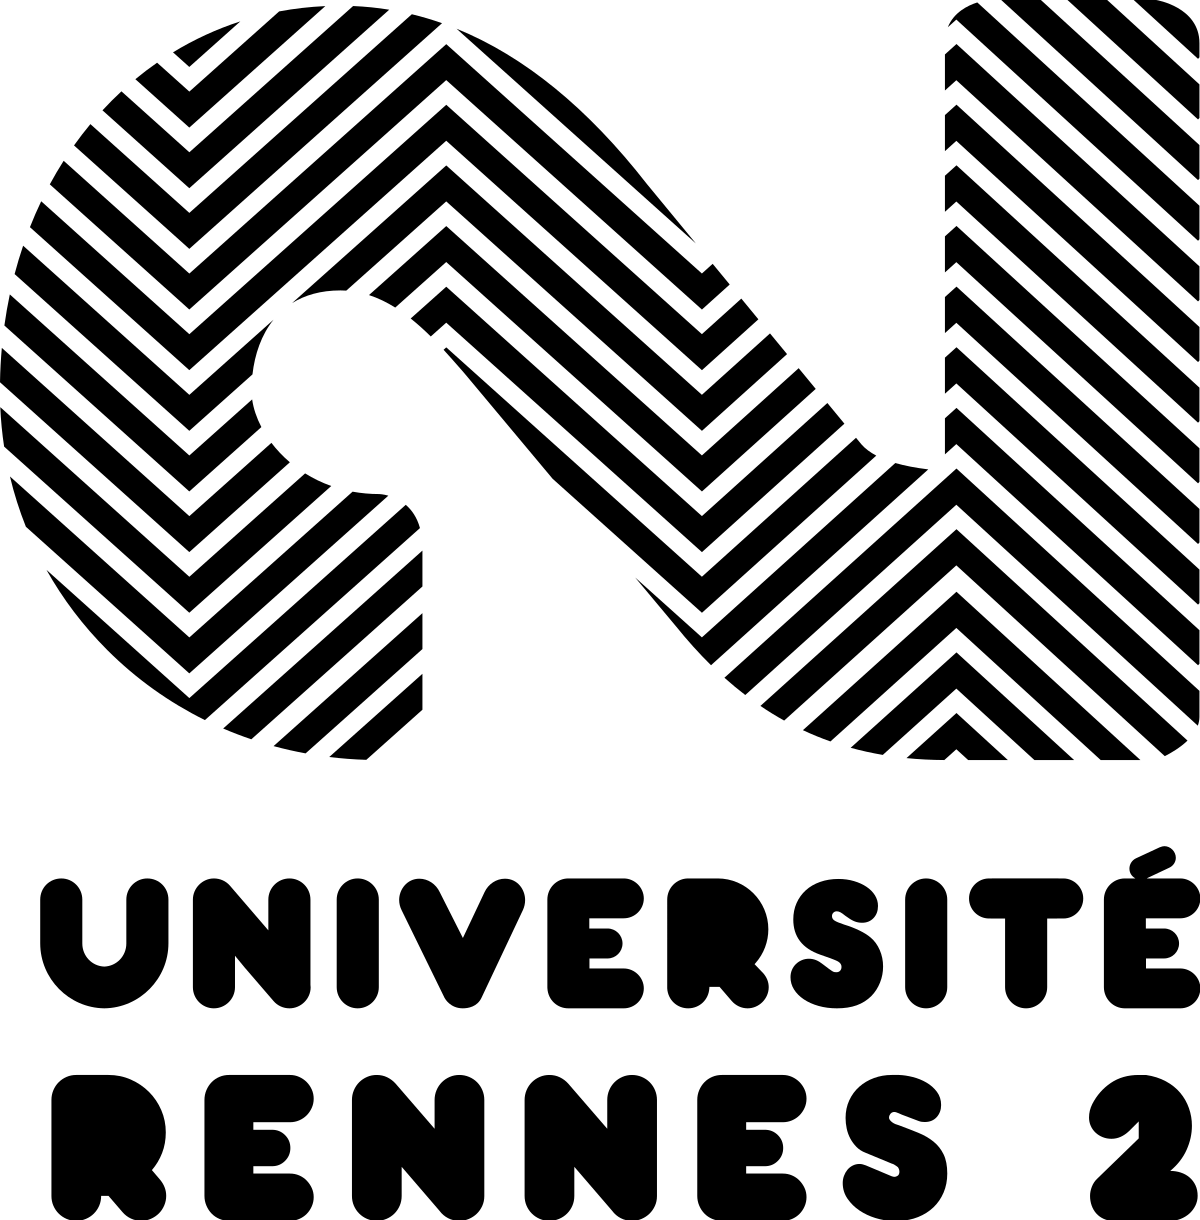
\includegraphics[scale=0.15]{Images/ur2.png}\\
\bigskip
\textsc{\Large Projet sur la fouille de données textuelles (\textit{Text Mining})}\\
    \HRule \\[0.4cm]
    { \huge \bfseries Wenger vs Mourinho : qu'en pense Twitter ?\\[0.4cm] }
        \HRule \\[2cm]
    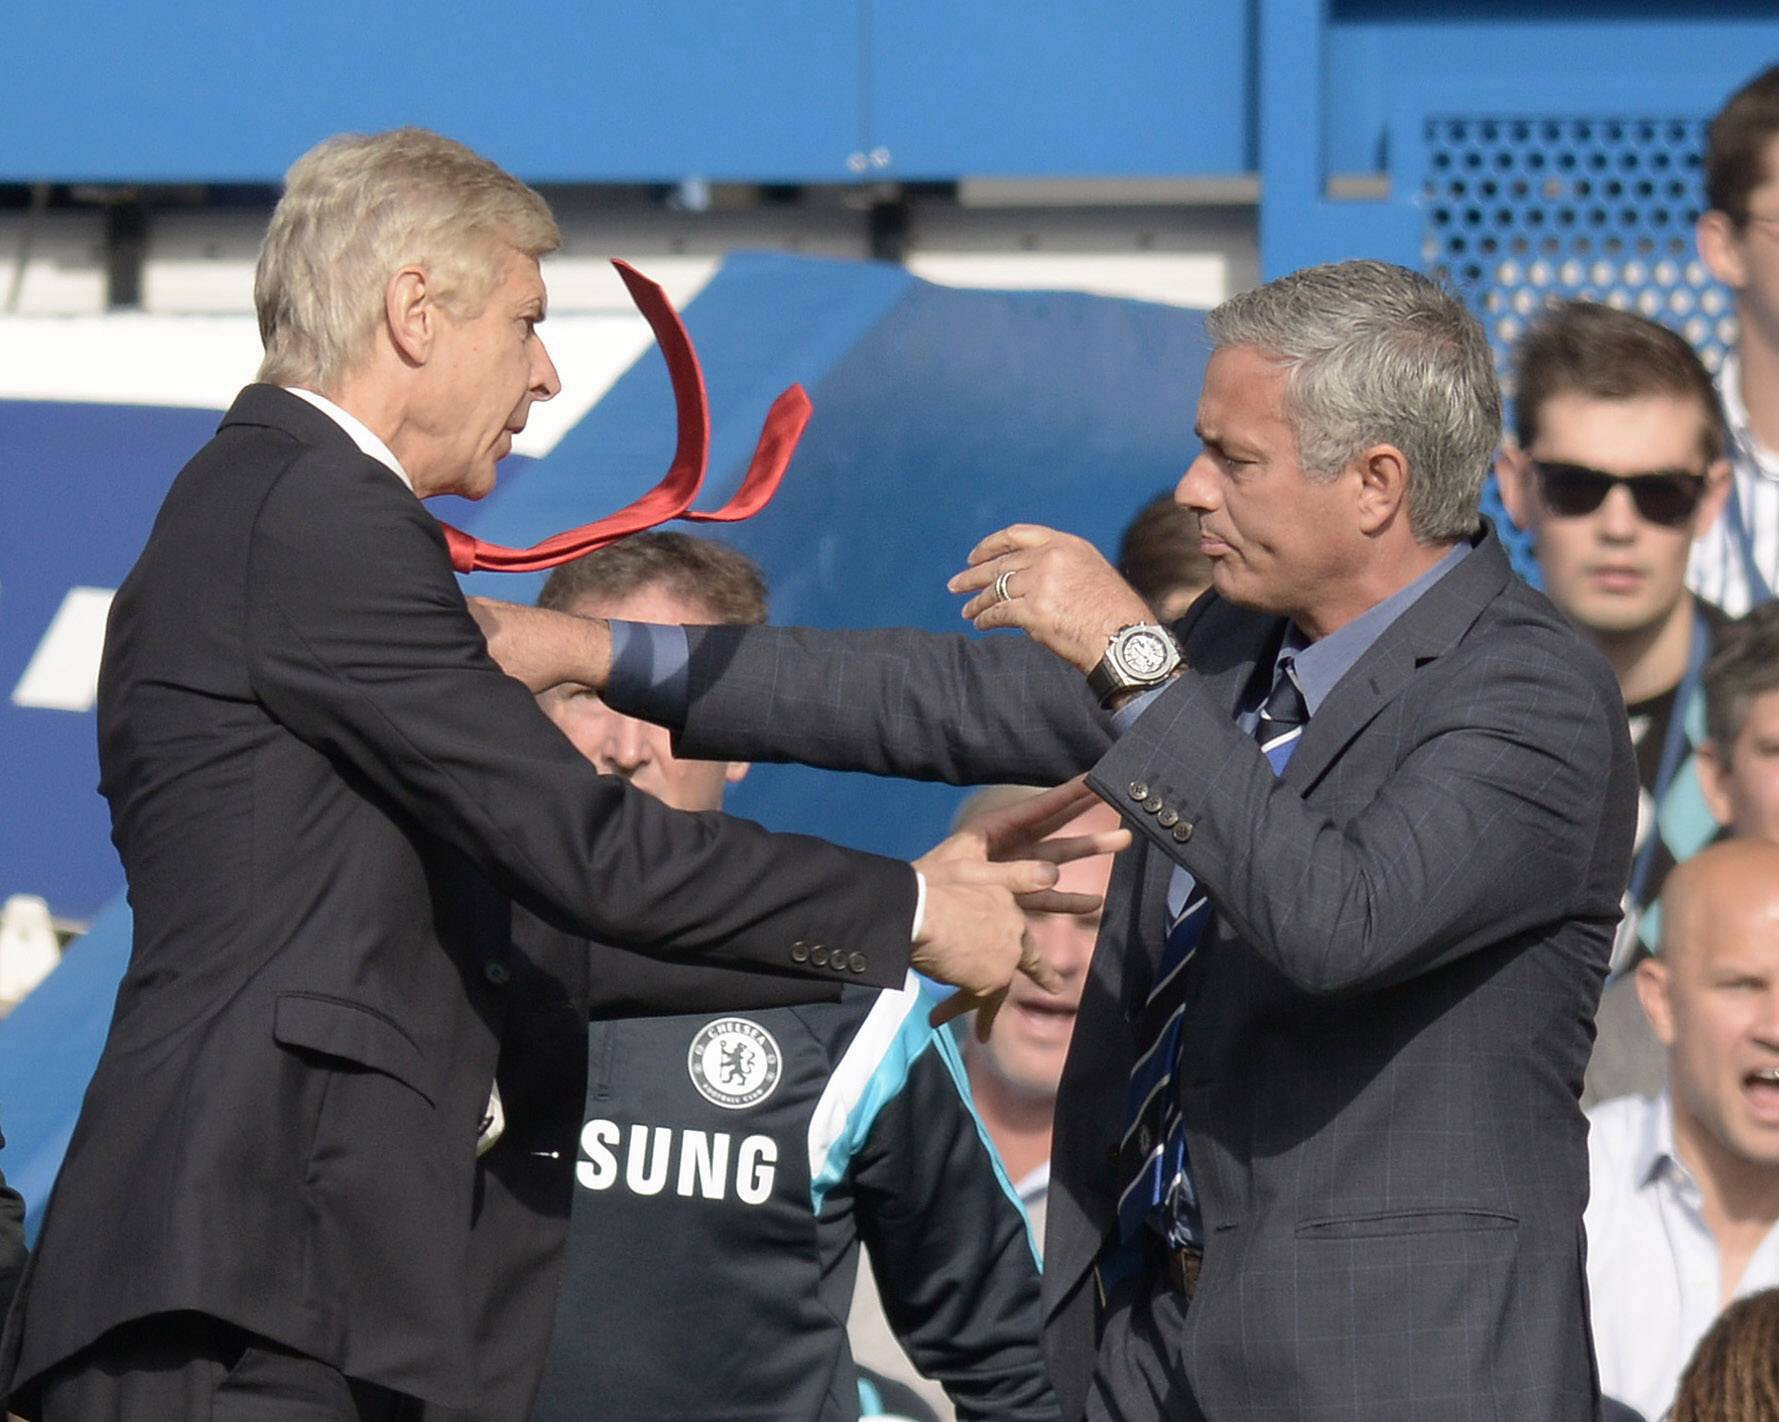
\includegraphics[scale=0.8]{Images/fight.jpg}
    \\[2cm]
    \begin{minipage}{0.4\textwidth}
      \begin{flushleft} \large
      	\textsc{Pierre BUREAU}\\
        \textsc{Guillaume LE FLOCH}\\
        Année 2017-2018\\
      \end{flushleft}
    \end{minipage}
    \begin{minipage}{0.4\textwidth}
      \begin{flushright} \large
        \emph{Encadrante : }\textsc{Mme Fabienne MOREAU}
      \end{flushright}
    \end{minipage}

    \vfill

\end{center}
\end{titlepage}
\tableofcontents

\newpage
\section{Introduction et problématique}
\paragraph{}
Tout amateur de football, et plus particulièrement du championnat anglais de \textbf{Premier League}, est au courant de la rivalité qui existe entre \textbf{Arsène Wenger} et \textbf{José Mourinho}. En effet, l'histoire entre nos deux protagonistes est riche en péripéties, faisons un bref rappel des faits.
\paragraph{}
Lorsque José Mourinho est nommé manager du club londonien de \textbf{Chelsea} à l'été 2004, Arsène Wenger sort d'une saison incroyable avec le club rival d'\textbf{Arsenal}, puisque les \textit{Gunners} ont remporté le championnat anglais sans avoir perdu le moindre match parmi les 38 journées sur lesquelles se déroule la Premier League. Arsenal termine donc champion avec \textbf{90 points}, c'est-à-dire 11 points de plus que le second... Chelsea !
\paragraph{}
On comprend ainsi qu'Arsène Wenger était à ce moment-là l'homme à abattre, et José Mourinho, qui sortait d'un doublé historique (Championnat du Portugal-Ligue des Champions) avec le \textbf{FC Porto} était l'élu pour accomplir cette tâche. Tout est fait pour opposer ces deux-là : l'entraîneur français est connu pour sa classe, pour donner leur chance aux jeunes joueurs, pour faire jouer son équipe avec un style \og léché \fg{} et offensif, quand son homologue portugais est décrit comme un grand tacticien, un entraîneur vicieux, au pragmatisme légendaire, qui s'appuie plutôt sur une défense de fer et des joueurs expérimentés. Mais ce n'est pas tout, José Mourinho est également un maître dans l'art de la provocation, pour déstabiliser l'adversaire. Il va ainsi lancer sans cesse des piques à Arsène Wenger ou Arsenal dans les médias, en conférence de presse avant ou après les matchs, ce qui va définitivement rendre la relation entre les deux managers tendue et mener à des altercations sur le bord du terrain lors des oppositions entre Arsenal et Chelsea, qui étaient déjà rivaux à la base. Chelsea terminera champion en 2005 et 2006, avant que Mourinho ne soit évincé. Il fera son retour à Chelsea en 2013, ce qui va raviver les tensions dans notre couple favori, remportera à nouveau la Premier League en 2015, puis sera à nouveau limogé 6 mois plus tard après une première partie de saison catastrophique. En 2016, il signe à Manchester United, autre rival historique d'Arsenal. L'histoire se poursuit donc encore aujourd'hui en 2018.
\paragraph{}
La situation actuelle est la suivante : Arsène Wenger est toujours en poste à Arsenal (depuis 1996) mais n'a plus remporté le championnat depuis cette fameuse saison 2003-2004. José Mourinho a terminé $6^{e}$ du championnat après avoir dépensé une fortune sur le marché des transferts pour bâtir son équipe. Cette saison, Manchester United et Arsenal n'arrivent pas à tenir la cadence infernale du Leader de Premier league, Manchester City, et sont à la traîne en championnat. Cela fait 14 ans qu'Arsenal n'a pas remporté le championnat, l'équipe commet tout le temps les mêmes erreurs, tandis que pour Mourinho son équipe est ennuyeuse à regarder jouer (à cause de sa tactique du \og \textit{park the bus} \fg{} qui consiste à défendre très bas en utilisant tous ses joueurs de champ et donc à \og garer le bus \fg{} devant son but pour empêcher l'adversaire de marquer), il n'a plus autant de succès qu'avant, c'est un \og chequebook-manager \fg{} (dans le sens où il ne bâtit son succès qu'en dépensant des sommes astronomiques pour attirer des grands joueurs, par opposition à Wenger qui développe des jeunes talents n'ayant quasiment rien coûté).
\paragraph{}
En bref, aujourd'hui ces deux managers sont très décriés, beaucoup de fans d'Arsenal et de Manchester United semblent vouloir le limogeage de leur manager respectif, en tout cas si l'on s'en fie à ce que l'on peut voir dans les journaux anglais ou sur les réseaux sociaux.
\paragraph{}
Nous avons donc décidé de nous pencher sur le cas de ces deux personnalités du monde du football et de vérifier si ces hypothèses sont vraies, en analysant les tweets dans lesquels ils sont mentionnés. Notre problématique sera la suivante : \textbf{Quelle est l'opinion des utilisateurs de Twitter vis-à-vis d'Arsène Wenger et de José Mourinho ?}
\paragraph{}
Cette problématique est assez large, et pour cette raison, notre étude va s'articuler en plusieurs étapes pour y répondre :
\begin{itemize}
\item Une analyse préliminaire des données afin de procéder à une sélection de tweets pertinents
\item Une analyse globale des tweets concernant chaque manager, afin de résumer les opinions
\item Une analyse plus détaillée pour tenter d'extraire de vraies tendances aux niveau des \textbf{hashtags} et de la \textbf{valeur sentimentale} des tweets
\end{itemize}
\newpage
\section{La récupération des données}
\paragraph{}
Une fois la problématique choisie, l'étape suivante de cette étude a été de construire notre base de données. Comme nous souhaitions analyser l'opinion des utilisateurs de \textbf{Twitter}, nous avons procédé au \textit{scraping} des tweets grâce à la librairie \textbf{tweepy} en Python, qui possède une API permettant de communiquer directement avec l'interface du célèbre réseau social.
\paragraph{}
Il est important de noter que l'extraction des tweets ne peut pas s'opérer sur des tweets anciens (c'est la réglementation de Twitter). Ce sont donc tous les tweets qui sont envoyés après le lancement du programme qui sont enregistrés et écrits dans un fichier au format \textit{json}. Ensuite, vous pouvez laisser votre programme tourner indéfiniment du moment que la connexion internet n'est pas coupée. Cependant, il existe des limitations (\textit{cf documentation complète dans les sources}) comme pour toute API. Pour notre cas particulier, les tweets qui ont été extraits contenaient soit le mot \og wenger \fg{} soit \og mourinho \fg{} (le code correspondant se trouve dans le script \textit{twitter\_streaming.py}). En ce qui nous concerne, l'extraction s'est faite en 4 fois pour plusieurs raisons :
\begin{itemize}
\item Il fallait un volume de données conséquent afin d'avoir suffisamment de tweets à analyser après avoir effectué un nettoyage complet
\item Nous ne pouvions pas laisser tourner le programme assez longtemps pour emmagasiner assez de tweets en une seule fois 
\item L'opinion des fans peut être biaisée à la suite d'un match perdu ou gagné par Arsenal et/ou Manchester United, nous avons donc souhaité capter des tweets à différents moments
\end{itemize}
Au final, nous nous retrouvons avec \textbf{1.60 Go} de données brutes à analyser, après agrégation des tweets extraits entre le \textbf{22 décembre 2017} et le \textbf{03 janvier 2018} (le code pour agréger les données correspond au script \textit{data\_concat.py}). Ces données sont regroupées dans un fichier texte appelé \textit{twitter\_data.txt}, qui est donc composé de tweets. Ces derniers sont au format \textit{json}, c'est à dire que ce sont des \textbf{dictionnaires} en Python. Ils renferment énormément d'informations et sont de la forme suivante :\\
\bigskip
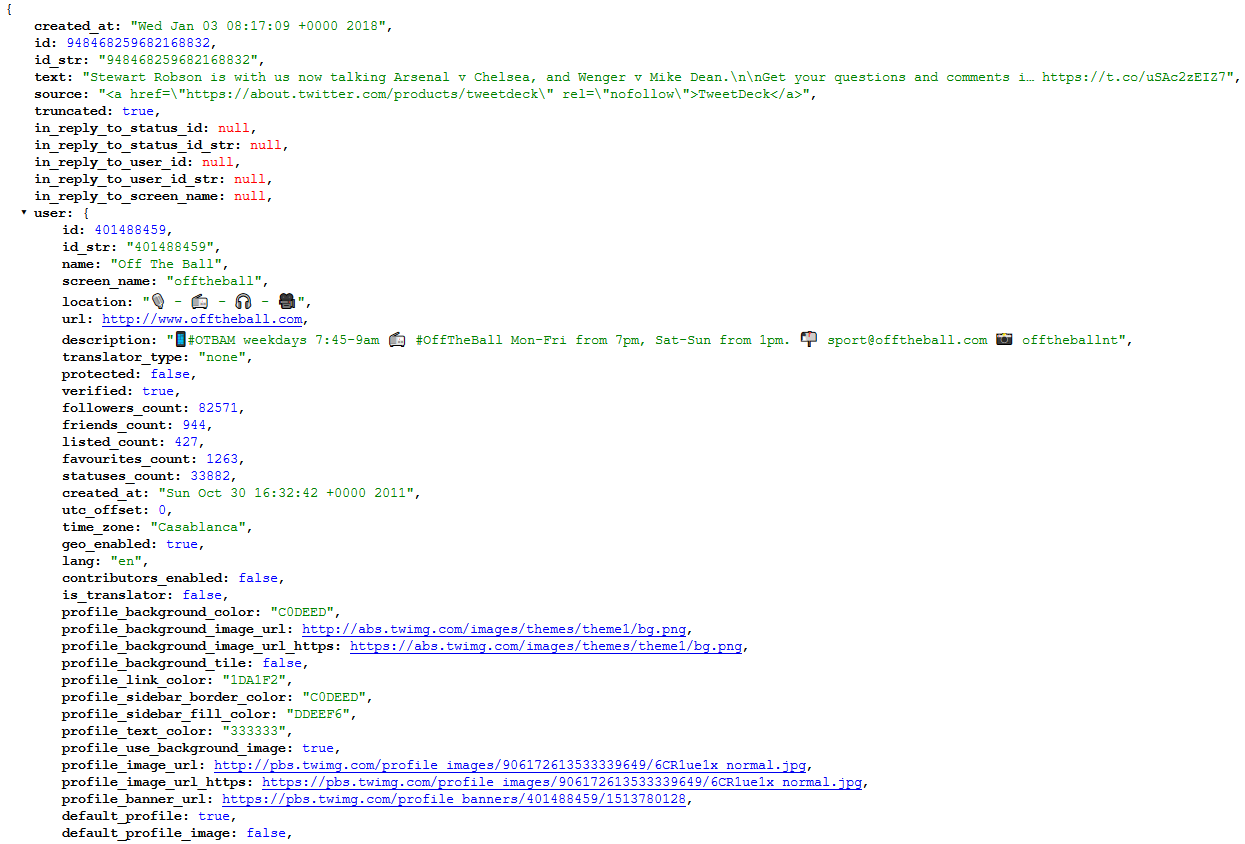
\includegraphics[scale=0.55]{Images/json_file.png}
\paragraph{}
Dans notre étude, nous allons nous servir principalement de la clé 'text' qui renferme le contenu des (désormais) 280 caractères maximum à disposition de l'utilisateur pour s'exprimer. La clé 'language' nous servira également dans l'analyse préliminaire pour sélectionner les tweets qui seront dans notre base finale à exploiter.
\section{Analyse préliminaire et nettoyage des données}
\paragraph{}
Extraire tous les tweets qui contiennent une chaîne de caractère donnée n'est pas compliqué, en revanche on peut se douter à l'avance que tout ne sera pas pertinent et que l'on va rencontrer certains problèmes. C'est pour cette raison qu'il nous fallait une base conséquente au départ, car elle va se retrouver largement affinée par la suite.
\paragraph{}
Un problème que nous n'avons pas eu, mais que nous aurions pu rencontrer concerne les différents sens du mot cible qui nous sert à effectuer l'extraction des tweets. Par exemple, si nous avions voulu nous pencher sur le cas de l'actuel manager de Chelsea, \textbf{Antonio Conte} et que nous avions seulement utilisé le mot clé \og conte \fg{} pour y faire référence, nous nous serions retrouvés avec des tweets parlant de personnes d'origine africaine portant le même nom, ou bien encore par exemple d'un \og conte de Noël \fg{}. Et si vous renseignez \og antonio conte \fg{} (l'API ne tient pas compte de la casse) vous ne pourrez extraire que les tweets contenant la chaîne complète, ce qui réduira donc largement le champs des tweets accessibles.
\paragraph{}
En ce qui nous concerne, il n'existe pas d'ambiguïté sur Mourinho et Wenger, ce sont des noms propres et aucune autre personnalité ne porte le même. En revanche, lorsque les fans ou journalistes parlent d'eux ils utilisent parfois \og Mou \fg{} ou \og José \fg{} pour parler de Mourinho et \og AW \fg{}, \og the Boss \fg{} ou encore \og Big Wengz \fg{} concernant Arsène Wenger. Nous n'avons donc pas pu capter tout ce qui se disait sur eux.
\paragraph{}
Néanmoins, nous avons réussi à extraire un total de \textbf{304 512} tweets. Un premier nettoyage a consisté à enlever les tweets pour lesquels il n'y avait pas de texte (ce qui correspond à une liste vide associée à la clé 'text' dans le dictionnaire python). En effet, un autre problème lié à la fouille de texte est que l'on ne peut pas exploiter les images, les GIFs ou encore les vidéos qui sont pourtant très porteurs de sens. Après avoir procédé à cette opération, il nous reste tout de même \textbf{304 488} tweets.
\paragraph{}
Un autre problème que l'on peut rencontrer avec les tweets est la présence de \textbf{doublons} ou de tweets qui sont quasiment des doublons. Cela concerne les fameux \textbf{retweets} : quand une personne va retweeter un tweet, cela va apparaitre sous la forme \og RT : blablabla \fg{}. Pour régler ce problème, nous avons donc décidé de supprimer tous les tweets commençant par \og RT \fg{}, on ne garde ainsi que le tweet original.\\
Le problème des \og quasi-doublons \fg{} était quant à lui dû aux liens (vers un article de presse par exemple) : on retrouve à chaque fois le même contenu textuel, mais puisque le lien est différent, la méthode \textit{drop\_duplicates()} de la librairie \textbf{Pandas} en Python ne détecte pas le doublon. La solution que nous avons choisie consiste tout simplement à supprimer au préalable tous les liens dans les tweets à l'aide d'une expression régulière.
\paragraph{}
Un autre aspect à prendre en compte est la langue dans laquelle est écrit le tweet. En effet, Arsenal et Manchester United sont des clubs de football suivis dans le monde entier, des fans de tous les pays tweetent à propos de ces 2 entités et de leurs managers. Nous avons donc décidé de regarder un \textit{Top 5} des langues dans lesquels nos tweets sont écrits.\\
\begin{center}
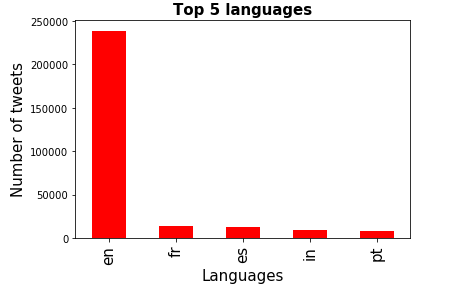
\includegraphics[scale=0.8]{Images/top5.jpg}
\end{center}
\paragraph{}
Les résultats sont sans appel, une écrasante majorité des tweets sont rédigés en anglais, ce qui n'est pas surprenant puisque la Premier League est beaucoup suivie au Royaume-Uni, en Amérique du Nord, en Inde et au Nigeria. Le français représente la deuxième langue, probablement grâce à Arsène Wenger et à la communauté francophone d'Arsenal. Cependant la quantité de tweets est insuffisante, puisque les doublons n'ont pas encore été enlevés. Nous allons donc conserver uniquement les tweets en anglais.
\paragraph{}
Après avoir effectué ces différentes opérations, nous allons stocker les tweets concernant José Mourinho dans un dataframe \textit{mourinho.csv}, idem pour Arsène Wenger (\textit{wenger.csv}). Au final, nous avons 26087 tweets pour José Mourinho et 28244 tweets pour Arsène Wenger, à analyser.
\section{Traitement global des tweets}

\section{Traitement détaillé des tweets}

\section{Bilan}

\section{Sources}
\begin{flushleft}
- \textbf{Réglementation de Twitter}, \href{https://developer.twitter.com/en/developer-terms/agreement-and-policy}{\textit{\textcolor{blue}{https://developer.twitter.com/en/developer-terms/agreement-and-policy}}}\\
\medskip
- \textbf{Scraping de tweets}, \href{https://marcobonzanini.com/2015/03/02/mining-twitter-data-with-python-part-1/}{\textit{\textcolor{blue}{https://marcobonzanini.com/2015/03/02/mining-twitter-data-with-python-part-1/}}}\\
\medskip
- \textbf{Analyse de sentiment}, \href{http://www.nltk.org/howto/sentiment.html}{\textit{\textcolor{blue}{http://www.nltk.org/howto/sentiment.html}}}\\
\end{flushleft}
\end{document}